\subsection{Budowa protokołu Bluetooth Low Energy}

\par
\tab \textbf{Opis protokołu} \\
\tab W rozdziale dotyczącym Bluetooth zostało wspomniane że Bluetooth Low Energy (lub Bluetooth Smart) jest protokołem nie do końca kompatybilnym z klasycznym Bluetooth-em. Wynika to z gruntownej przebudowie jakiej został poddany Bluetooth aby stworzyć BLE, głównymi zmianami jest: skorzystanie z nowej modulacji (GFSK) w warstwie fizycznej oraz gruntownej przebudowie warstwy sieciowej, wszystko w celu "odchudzenia" i umożliwienia implementacji standardu BLE urządzenią o ograniczonej mocy obliczeniowej. \\
Tym co jednak zostało nie zmienione w BLE są wyższe warstwy protokołu takie jak ATT czy L2CAP.\\
Bluetooth Low Energy znajdziemy między innymi w Nowych smartphonach, urządzeniach i gadżetach sportowych, inteligentnych zamkach czy nawet niekiedy w urządzeniach medycznych.\\

\par
\tab \textbf{Budowa warstwowa BLE} \\ 
\tab Jak zostało wcześniej powiedziane wyższe warstwy protokołu są takie same jak w Bluetooth tzn: znajdują się tutaj warstwa GATT, ATT, L2CAP. Dodatkowo są niższe warstwy związane z samą transmisją tzn: warstwa Fizyczna (PHY) oraz sieciowa (Link Layer).\\

\centerline{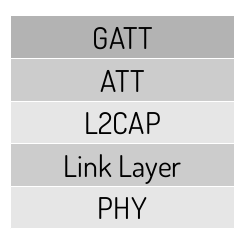
\includegraphics[scale=0.5]{./img/BLE_Stack.png}}

W skład widma 2.4GHz wchodzi 40 kanałów z tego 37 kanałów do wymiany danych oraz 3 kanały służące do rozgłasania się. BLE implementuje również mechanizm tzn: Hopping-u, czyli w trakcie transmisji zmiany kanału na którym odbywa się transmisja.\\

\par
\tab \textbf{Architektura sieci} \\ 
Wszystkie urządzenia korzystające z Bluetooth LE mogą pełnić jedną z dwóch roli: Master lub Slave (czasem również spotykane Client, Server). Master może nawiązywać połączenia z wieloma slavami natomiast slave jedynie czeka na nawiązanie transmisji (nie może zainicjalizować samodzielnie połączenia). \\
Obiektem kluczowym w całej komunikacji jest tzw. GATT (GATT)  czyli profil urządzenia który zawiera informacje i interfejs jaki urządzenie (serwer) udostępnia na zwenątrz. \\
W skład profilu GATT może wchodzić wiele serwisów natomiast każdy serwis może się składać z kilku charakterystyk. Charakterystyka jest obiektem (wartością) którą można zapisać lub odczytać do urządzenia.\\
Poniżej zaprezentowany jest schemat budowy profilu GATT i zależności między profilem-serwisem i charakterystyką. \\

\centerline{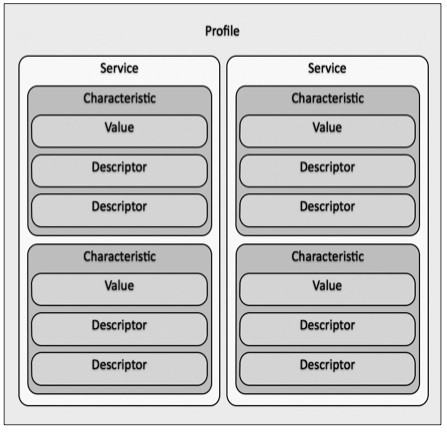
\includegraphics[scale=0.5]{./img/GATT_char_ble.jpg}}

\par
\tab \textbf{Profile BLE} \\
Bluetooth Smart wprowadza w ramach standardu szereg profili (GATT) gotowych do użycia w min następujących aplikacjach:
\begin{enumerate}
	\item Health care profiles
	\item Sports and fitness profiles
	\item Internet Connectivity
	\item Generic Sensors
	\item HID Connectivity
	\item Internet Connectivity
\end{enumerate}  


\clearpage